\documentclass[11pt]{article}

\usepackage[T1]{fontenc}
\usepackage{newtxtext}
\usepackage{newtxmath}
\usepackage{amsmath}
\usepackage{amssymb}
\usepackage[margin=1in]{geometry}
\usepackage{natbib}
\usepackage{enumitem}
\usepackage{booktabs}
\usepackage{graphicx}
\usepackage{hyperref}
\usepackage{float}

\setlength{\parindent}{0pt}
\setlength{\parskip}{0.5em}
\setlist[itemize]{leftmargin=1.3em,itemsep=0.2em,topsep=0.2em}
\setlist[enumerate]{leftmargin=1.5em,itemsep=0.2em,topsep=0.2em}

\begin{document}

{\Large\bfseries Resampling-Based Model Selection for PE SDFs\par}
{\normalsize How to empirically measure the risk-adjusted performance of non-traded cash flows\par}
\today

\section{Idea}

The paper asks a simple empirical question: which stochastic discount factor (SDF) models give the most credible risk adjustment for private-equity cash flows?

Three difficulties make this question hard to answer with existing methods.

\textbf{Difficulty 1: moment construction matters.}
Private-equity samples are small, lumpy, and organized by vintage year. An SDF model can look good or bad depending on how funds are grouped into pricing moments. Existing approaches commit to one grouping---typically single funds (e.g., \cite{AngChenGoetzmannPhalippou2018}) or vintage-year portfolios (e.g., \cite{DriessenLinPhalippou2012})--and treat it as fixed. But the choice of grouping is itself consequential for estimation, and there is no a priori reason to prefer one admissible grouping over another.

\textbf{Difficulty 2: unseasoned vintages create a dilemma.}
Recent vintage years carry valuable pricing information---they reflect current market conditions and expand the factor-path coverage of the sample---but including them naively destabilizes (or biases) estimation. The standard approach treats the latest reported NAV as a terminal cash flow and discounts it over the fund's entire remaining horizon. This creates two problems. First, it concentrates a large share of the fund's discounted value at a single calendar date---the dataset endpoint---so that the estimator's fit becomes disproportionately sensitive to the macro state at that date rather than to the fund's lifetime factor exposure. Second, the terminal NAV is an appraisal, not a realized payoff; its co-movement with public indices may differ systematically from that of actual divestitures. Researchers therefore face a dilemma: exclude recent vintages and waste data, or include them and accept fragile estimates driven by one macro-state realization.

\textbf{Difficulty 3: exploding-alpha degeneracy in finite samples.}
Independently of the unseasoned-vintage problem, NPV-style SDF estimation suffers from a finite-sample pathology first documented by \citet{DriessenLinPhalippou2012}. In the standard multiplicative SDF parameterization, cash flows are discounted by a cumulative factor that includes \((1+\alpha)^{-T}\). When \(\alpha\) is large and positive, this factor drives all discount factors toward zero for large \(T\), making every fund's pricing error approximately zero regardless of the factor loadings~\(\beta\). The result is a ridge of spurious near-minima along the alpha axis of the objective function that prevents reliable joint identification of \(\alpha\) and~\(\beta\). The problem is most severe when fund horizons are long and early cash flows are small relative to later ones, which is precisely the cash-flow shape of a typical PE fund. Existing mitigants include ratio or log transformations of the pricing restriction \citep{DriessenLinPhalippou2008WP}, horizon averaging, and box constraints on~\(\alpha\), but none eliminates the underlying mechanism.

We propose a \emph{hybrid cash-flow / normalized-Euler estimator} that addresses all three difficulties. The estimator has two components:

\begin{enumerate}
\item \textbf{Hybrid pricing restrictions.} For seasoned vintages whose funds are substantially liquidated, the estimator uses the standard cumulative cash-flow pricing error. For unseasoned vintages with significant residual NAVs, it replaces the single long-horizon pricing restriction with a sequence of one-period Euler restrictions on quarterly NAV returns. Each quarterly Euler error is normalized by lagged capital at risk and then rescaled by an exogenous duration factor so that the resulting young-fund moment is expressed in NPV-like units per committed dollar. Because the quarterly block uses only one-period SDF terms, its sensitivity to alpha is proportional to the quarter length rather than exponential in the fund horizon. Under increasing-domain asymptotics, only a vanishing fraction of vintages uses this normalized Euler block, so the estimator becomes asymptotically cash-flow dominated.
\item \textbf{Resampling-based model selection.} Instead of committing to one grouping of funds into pricing moments, we make the grouping itself part of the empirical design. We repeatedly draw random within-vintage fund partitions, estimate the SDF on partition-induced moments, and evaluate pricing errors on held-out moments. The preferred SDF model is the one with the lowest average holdout pricing loss across many admissible partitions.
\end{enumerate}

The method therefore has three goals:

\begin{itemize}
\item \textbf{Efficient use of the vintage panel:} include all available vintages---seasoned and unseasoned---without triggering exploding-alpha instability.
\item \textbf{Model selection:} rank SDF models by out-of-sample pricing performance across many resampled moment constructions.
\item \textbf{Design comparison:} compare whether within-vintage fund resampling or traditional vintage-year portfolio construction yields more stable and predictive pricing moments.
\end{itemize}

The paper is closest in spirit to \citet{KortewegNagel2016} because the estimator works with aggregated pricing moments, and to \citet{DriessenLinPhalippou2012} because the moments price private cash flows directly. The new contributions are the hybrid CF/normalized-Euler pricing restriction for young vintages, and the resampling layer that treats moment construction as a testable design choice rather than a fixed input.
\cite{brown2023nowcasting} also use NAVs to estimate the risk and return of PE funds.

\section{Guiding Example}

Suppose a candidate SDF has three parameters: an alpha term and two factor loadings. Then we need at least three pricing moments to estimate it. A natural resampling design is therefore:

\begin{itemize}
\item build three estimation folds,
\item build one validation fold,
\item estimate the SDF on the three estimation moments,
\item score the fitted SDF on the validation moment (calculate out-of-sample pricing error).
\end{itemize}

In stylized notation, the example can be summarized with one simple three-parameter SDF and one resampled moment per fold. Let the parameter vector be
\[
\theta=(\alpha,\beta_1,\beta_2)^\prime,
\]
and let the one-period discount factor be
\[
M_{t-1,t}(\theta)=\frac{1}{1+\alpha+\beta_1 f_{1,t}+\beta_2 f_{2,t}},
\qquad
\Psi_{0,t}(\theta)=\prod_{s=1}^{t} M_{s-1,s}(\theta),
\]
where \(f_{1,t}\) and \(f_{2,t}\) are two benchmark factor realizations. For sampled split \(n\), let \(C_{n,v,r}\) be the funds from vintage \(v\) assigned to fold \(r\in\{1,2,3,4\}\), with \(r=1,2,3\) used for estimation and \(r=4\) used for validation. Write \(CF_{t,i}=D_{t,i}-X_{t,i}\), and partition active vintages into seasoned and unseasoned sets, \(\mathcal V=\mathcal V^S\cup\mathcal V^U\). The vintage-level pricing restriction is then
\[
\epsilon_{n,v,r}(\theta)=
\begin{cases}
\epsilon_{n,v,r}^{S}(\theta)
=
\dfrac{1}{|C_{n,v,r}|}
\sum\limits_{i\in C_{n,v,r}}
\dfrac{1}{K_i}
\sum\limits_{t=1}^{T_i}
\Psi_{0,t}(\theta)\,CF_{t,i},
& v\in\mathcal V^S,
\\[1.1em]
\epsilon_{n,v,r}^{U}(\theta)
=
\dfrac{1}{|C_{n,v,r}|}
\sum\limits_{i\in C_{n,v,r}}
\Lambda_i\,
\dfrac{1}{T_i}
\sum\limits_{t=1}^{T_i}
\dfrac{\eta_{t,i}(\theta)}{s_{t-1,i}},
& v\in\mathcal V^U,
\end{cases}
\]
where the unseasoned one-period Euler error is
\[
\eta_{t,i}(\theta)
=
M_{t-1,t}(\theta)\bigl(CF_{t,i}+\mathrm{NAV}_{t,i}\bigr)-\mathrm{NAV}_{t-1,i}.
\]
Here \(s_{t-1,i}=\max\{\mathrm{NAV}_{t-1,i},\nu K_i\}\) converts each quarterly Euler error into a relative error per dollar at risk, while \(\Lambda_i\) is a predetermined duration-matching normalizer based on fund age and strategy that maps the fund-average relative Euler error into an NPV-like quantity per committed dollar.
The resampled fold moment is the cross-vintage average
\[
m_{n,r}(\theta)=\frac{1}{|\mathcal V|}\sum_{v\in\mathcal V}\epsilon_{n,v,r}(\theta).
\]
Because \(\theta\) has three components, the three estimation folds deliver three stylized moment conditions,
\[
m_{n,1}(\theta)=0,
\qquad
m_{n,2}(\theta)=0,
\qquad
m_{n,3}(\theta)=0,
\]
or equivalently
\[
\hat\theta_n
=
\arg\min_{\theta}
\sum_{r=1}^{3} m_{n,r}(\theta)^2.
\]
The held-out fourth fold then gives the validation score
\[
S_n(\hat\theta_n)=m_{n,4}(\hat\theta_n)^2.
\]
Our resampling-based approach repeats this exercise many times: for each draw \(n=1,\dots,N\), we redraw the partition and thereby obtain a new quartet of fold moments \(\{m_{n,1},m_{n,2},m_{n,3},m_{n,4}\}\).

Figures \ref{fig:sampling-scheme} and \ref{fig:vintage-portfolio-scheme} show the two baseline ways to build these folds. In both figures, each dot is one fund. Vintages 2005--2010 lie above the approach boundary and use cash-flow discounting, while vintages 2011--2012 lie below it and use the normalized Euler approach.

\begin{figure}[H]
\centering
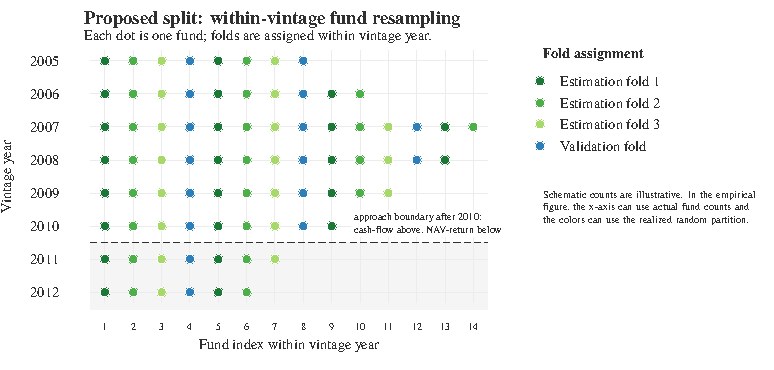
\includegraphics[width=\linewidth]{../figure/sampling_scheme.pdf}
\caption{Proposed within-vintage fund resampling scheme. Each active vintage is split into three estimation cells and one validation cell. Fold 1 contains the dark-green funds from every vintage, fold 2 contains the medium-green funds from every vintage, fold 3 contains the light-green funds from every vintage, and the validation fold contains the blue funds from every vintage.}
\label{fig:sampling-scheme}
\end{figure}

\begin{figure}[H]
\centering
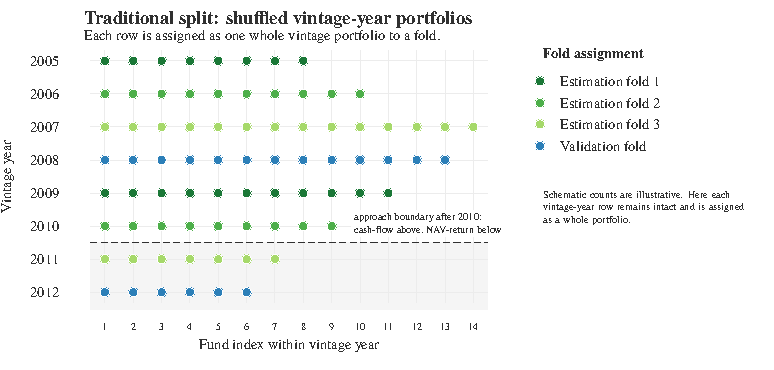
\includegraphics[width=\linewidth]{../figure/sampling_scheme_vintage_portfolios.pdf}
\caption{Traditional shuffled vintage-year portfolio scheme. Funds are first aggregated into whole vintage-year portfolios, and whole vintages are then assigned to folds. Here, 2005 and 2009 enter estimation fold 1, 2006 and 2010 enter estimation fold 2, 2007 and 2011 enter estimation fold 3, and 2008 and 2012 form the validation fold.}
\label{fig:vintage-portfolio-scheme}
\end{figure}

\section{Two Canonical Sampling Schemes}

\textbf{Proposed split: within-vintage fund resampling.}
In the proposed design, every fold contains funds from every active vintage. This keeps the vintage-year support fixed across estimation and validation moments. The folds differ because they contain different funds, not because they represent different macro or vintage states. This is the cleanest design for asking whether an SDF prices PE cash flows robustly across fund-level resamples.

\textbf{Benchmark split: shuffled vintage-year portfolios.}
In the traditional design, the primitive object is a vintage-year portfolio. A fold contains whole vintages, not fund sub-samples from all vintages. This is easy to explain and resembles standard PE portfolio construction. But the validation moment now differs from the estimation moments in vintage composition. A failure on the validation fold may therefore reflect poor SDF pricing, or it may reflect extrapolation across vintage states.

The first version of the paper should focus on this contrast. If within-vintage resampling delivers more stable estimates and lower holdout pricing errors, the evidence favors building all-vintage subportfolios before estimating the SDF. If shuffled vintage-year portfolios perform similarly, the simpler vintage-year construction may be sufficient.

\section{Objects and Notation}

Let \(v=1,\dots,V\) index active vintage years, and let \(\mathcal I_v\) be the set of funds in vintage \(v\). Let \(M\) denote a candidate SDF model with parameter vector \(\theta\in\Theta_M\subset\mathbb R^{p(M)}\).

We use \(P\) estimation folds and \(h\) holdout folds. For the guiding three-parameter example, \(P=3\) and \(h=1\). When comparing models with different numbers of parameters, a clean implementation is to use a common number of estimation folds \(P=p_{\max}\), where \(p_{\max}=\max_M p(M)\).

\subsection{Within-vintage resampling}

For sampled split \(n=1,\dots,N\), split the funds within each vintage into \(P+h\) cells:
\[
\mathcal P_{n,v}
=
\{C_{n,v,1},\dots,C_{n,v,P+h}\},
\qquad
C_{n,v,r}\subset \mathcal I_v.
\]
The cells are disjoint and cover the funds in vintage \(v\). The \(r\)th cross-vintage fold is
\[
F_{n,r}
=
\{C_{n,1,r},C_{n,2,r},\dots,C_{n,V,r}\}.
\]
Thus fold \(r\) contains one fund sub-sample from every active vintage.

At the single-fund level, the number of admissible assignments is usually too large to enumerate. We therefore draw Monte Carlo samples from a partition rule \(\Pi\):
\[
\mathcal P_n
\sim
\Pi(\cdot \mid P,h,\mathcal I_1,\dots,\mathcal I_V).
\]
For now, \(\Pi\) should be simple and transparent: random assignment within each vintage, subject to no empty cells and reasonable balance in fund counts or economic size.

\subsection{Vintage-year portfolio benchmark}

For the benchmark design, first aggregate all funds in each vintage \(v\) into a vintage-year portfolio. Then assign whole vintages to folds. The notation is the same at the fold level, but the economic object differs: \(F_{n,r}\) now contains whole vintage-year portfolios rather than within-vintage fund cells.

\section{Pricing Moments}
\label{sec:pricing_moments}

For a fold \(F_{n,r}\), let \(\epsilon_{n,v,r}(\theta;M,\eta)\) be the pricing error from the vintage component of that fold. The design choice \(\eta\) collects choices such as the alpha definition, loss function, and cash-flow weighting.

The aggregated fold moment is
\[
m_{n,r}(\theta;M,\eta)
=
\sum_{v\in A_{n,r}}
\omega_{n,v,r}\,
\epsilon_{n,v,r}(\theta;M,\eta),
\]
where \(A_{n,r}\) is the set of vintages represented in fold \(r\), and \(\omega_{n,v,r}\) are vintage or value weights. Under within-vintage resampling, \(A_{n,r}\) is the full active vintage set for every fold. Under shuffled vintage-year portfolios, \(A_{n,r}\) is only the set of whole vintages assigned to fold \(r\).

This distinction is the core empirical design choice. The proposed method creates comparable fold moments that all span the same vintage domain. The benchmark creates moments from different vintage domains.

\subsection{Fund weights and vintage weights}
\label{sec:fund_vintage_weights}

The fund-level scaling and vintage weight are design choices that determine the economic content of the fold moment. For seasoned funds, the baseline contribution is
\[
g_i^S(\theta;M,\eta)=\frac{1}{K_i}\sum_{t=0}^{T_i}\Psi_{0,t}(\theta;M,\eta)\,CF_{t,i},
\]
so each seasoned fund contributes a \emph{relative} NPV error per dollar committed. For unseasoned funds, the analogous baseline contribution is the normalized Euler error \(g_i^U(\theta;M,\eta)\) defined in Section~\ref{sec:euler_nav}: a fund-average one-period Euler error scaled by lagged capital at risk and rescaled by a deterministic duration factor. At the cell level, we average over the funds in the cell. At the vintage level, the baseline sets \(\omega_{n,v,r}=1/|A_{n,r}|\) (equal vintage weights), so that each vintage contributes equally to the fold moment regardless of the number of funds or aggregate capital it contains.

Under this hybrid three-layer normalization (fund \(\to\) cell \(\to\) vintage), the fold moment becomes
\[
m_{n,r}(\theta;M,\eta)
=
\frac{1}{|A_{n,r}|}
\left[
\sum_{v\in\mathcal V^S\cap A_{n,r}}
\frac{1}{|C_{n,v,r}|}\sum_{i\in C_{n,v,r}} g_i^S(\theta;M,\eta)
\;+\;
\sum_{v\in\mathcal V^U\cap A_{n,r}}
\frac{1}{|C_{n,v,r}|}\sum_{i\in C_{n,v,r}} g_i^U(\theta;M,\eta)
\right].
\]
This is an average, across vintages, of the average relative pricing error per fund. For seasoned vintages the object is a relative NPV error; for unseasoned vintages it is a duration-matched relative Euler error expressed in comparable per-committed-dollar units. It is therefore comparable across: (i)~vintages with different numbers of funds, (ii)~vintages with different aggregate capital, (iii)~seasoned vintages with cash-flow errors and unseasoned vintages with normalized Euler errors (Section~\ref{sec:euler_nav}), and (iv)~estimation folds and validation folds.

\section{Estimation and Holdout Scoring}

For each sampled split \(n\), let \(E_n\) be the set of estimation folds and \(H_n\) the validation fold. The split-specific estimator solves
\[
\hat\theta_n(M,\eta,\Pi)
=
\arg\min_{\theta\in\Theta_M}
\frac{1}{P}\sum_{j\in E_n}
L\!\left(m_{n,j}(\theta;M,\eta)\right).
\]

The validation score is the pricing loss on the held-out fold:
\[
S_n(M,\eta,\Pi)
=
L\!\left(m_{n,H_n}(\hat\theta_n(M,\eta,\Pi);M,\eta)\right).
\]

Aggregate this score across many sampled assignments:
\[
\mathrm{Score}_N(M,\eta,\Pi)
=
\frac{1}{N}\sum_{n=1}^{N} S_n(M,\eta,\Pi).
\]

The preferred model-design pair \((M,\eta,\Pi)\) is the one with the lowest average holdout pricing loss. Parameter stability is still informative, but the primary ranking criterion should be predictive pricing performance: does the fitted SDF price cash flows that were not used in estimation?

\subsection{Choice of Pricing Moment}
\label{sec:moment_choice}

The pricing error \(m_{n,j}(\theta;M,\eta)\) in the loss \(L\) is a design choice,
not a primitive. Two canonical families appear in the private-capital SDF
literature: the \emph{dollar NPV} moment of \citet{DriessenLinPhalippou2012}
and the \emph{PME-ratio} moment of \citet{KaplanSchoar2005},
\citet{DriessenLinPhalippou2009}, and \citet{AngChenGoetzmannPhalippou2018}.
Because the resampling-based ranking of \((M,\eta,\Pi)\) can in principle be
sensitive to this choice, we discuss both here and treat the NPV moment as
the baseline, the PME-ratio as a robustness check.

\paragraph{Dollar NPV moment.}
For seasoned funds in fold cell \(j\) in split \(n\), aggregate discounted cash flows into one
cumulative pricing error,
\[
m^{\mathrm{NPV}}_{n,j}(\theta;M,\eta)
=\sum_{i\in C_{n,j}} w_i\sum_{t=0}^{T_i}\Psi_{0,t}(\theta;M,\eta)\,CF_{t,i},
\qquad CF_{t,i}=D_{t,i}-X_{t,i},
\]
where \(X_{t,i}\) are contributions, \(D_{t,i}\) distributions (including
terminal NAV for seasoned funds), and \(\Psi_{0,t}\) the cumulative SDF. At
the population parameter, \(E[m^{\mathrm{NPV}}_{n,j}(\theta_0)]=0\): the
risk-adjusted NPV of fund cash flows vanishes.

For unseasoned funds, we do \emph{not} append the latest NAV as a terminal distribution and discount it to time zero. Instead, the operational baseline replaces each young fund's contribution with the normalized Euler fund moment \(g_i^U(\theta;M,\eta)\) from Section~\ref{sec:euler_nav}. The empirical baseline is therefore hybrid: cumulative NPV for \(\mathcal V^S\), normalized Euler for \(\mathcal V^U\).

\emph{Pros.}
(i)~\emph{Linearity} in cash flows yields tractable GMM derivatives,
influence functions, and CLT-based inference.
(ii)~\emph{Additivity} across funds makes the fold structure of
Section~\ref{sec:algorithm}, as well as subsampling and the bootstrap,
transparent: the cell moment is the sum of fund-level moments, and the split
moment is the sum of cell moments.
(iii)~\emph{Compatibility with the normalized Euler NAV restriction} for
unseasoned vintages: the seasoned block remains a linear cash-flow NPV,
while the unseasoned block uses lagged-scale one-period Euler errors rescaled
by an exogenous duration factor. Both blocks are expressed as per-committed-dollar
pricing errors, and neither requires ratio denominators that can approach zero.

\emph{Cons.}
(i)~\emph{Scale-dependence.} A \$1B fund with a 1\% relative NPV error
contributes ten times more to the moment than a \$100M fund with the same
relative error, so efficient GMM weighting implicitly tilts the estimator
toward mega-funds. The influence function is mechanically heavy-tailed in
the fund-size distribution rather than in genuine pricing disagreement.
(ii)~\emph{Dollar-denominated comparisons across vintages} with
heterogeneous aggregate commitments are not directly meaningful; normalization
is left to the econometrician.
(iii)~\emph{Sign cancellation.} A cross-sectional mean of zero is consistent
with systematic under-pricing of one subgroup offsetting over-pricing of
another, which the scalar moment cannot detect. This motivates the
fine-grained fold structure but does not eliminate the concern within a
fold.

\paragraph{PME-ratio moment.}
Define the risk-adjusted PME of fund \(i\) as
\[
\mathrm{PME}_i(\theta;M,\eta)
=\frac{\sum_{t}\Psi_{0,t}(\theta;M,\eta)\,D_{t,i}}
{\sum_{t}\Psi_{0,t}(\theta;M,\eta)\,X_{t,i}},
\]
from which two natural cell-level moments follow: the \emph{average-PME}
form
\(
m^{\mathrm{PME}}_{n,j}(\theta)
=|C_{n,j}|^{-1}\sum_{i\in C_{n,j}}\bigl(\mathrm{PME}_i(\theta)-1\bigr)
\)
and the \emph{pooled-PME} form
\(
m^{\mathrm{PME\text{-}pool}}_{n,j}(\theta)
=\bigl(\sum_{i,t}\Psi_{0,t}D_{t,i}\bigr)/\bigl(\sum_{i,t}\Psi_{0,t}X_{t,i}\bigr)-1.
\)
Both have mean zero at \(\theta_0\) under standard regularity, but they
estimate different population objects (mean of a ratio versus ratio of
means).

\emph{Pros.}
(i)~\emph{Scale-invariance.} The ratio is unit-free, so fund-size
heterogeneity does not mechanically up-weight mega-funds. A \$100M fund and
a \$1B fund enter the cross-sectional moment on equal footing.
(ii)~\emph{Practitioner interpretability.} PME is the native performance
metric of the industry; reporting results in the same units aids
dissemination.
(iii)~\emph{Bounded downside.} The fund-level PME is bounded below by zero,
so \(\mathrm{PME}_i-1\) is bounded below by \(-1\): a single disaster fund
cannot dominate the moment the way it can dominate a dollar NPV.

\emph{Cons.}
(i)~\emph{Nonlinearity.} The moment is a ratio in \(\theta\); its derivative
involves the ratio of two correlated sums and is numerically fragile when
the denominator (discounted contributions) is small. This occurs
mechanically for young funds with back-loaded capital calls --- precisely
the vintages that the Euler NAV restriction is designed to retain.
(ii)~\emph{Jensen-style bias between forms.} The average-PME and pooled-PME
moments can differ in finite samples by a term of order
\(\mathrm{Var}(X_i)/\bar X^2\); the two are asymptotically equivalent only
under degenerate size distributions. Researchers must commit to one and
defend it.
(iii)~\emph{No clean short-horizon analogue for unseasoned vintages.}
Integrating unseasoned vintages \(\mathcal V^U\) into a PME framework typically
requires treating the latest \(\mathrm{NAV}_{T_i,i}\) as a terminal distribution
and discounting it over the fund's entire remaining horizon --- exactly the
long-horizon discounting mechanism that the normalized Euler block is designed
to avoid.
%The PME-ratio framework therefore reintroduces the exploding-alpha sensitivity for \(\mathcal V^U\) that the NPV/Euler combination was designed to eliminate.
(iv)~\emph{Inference.} Upper-tail skewness in \(\mathrm{PME}_i\) (funds can
return many times their capital, but cannot lose more than it) distorts
CLT-based standard errors and \(t\)-statistics unless explicitly
robustified, e.g., by bootstrapping the cell-level moment or by employing
median-based loss functions.

\paragraph{Choice for the empirical implementation.}
The tractability of the seasoned NPV block and the stability of the normalized
Euler block make the hybrid NPV/Euler construction our primary analytical
framework. The seasoned contribution is a relative NPV error per dollar
committed; the unseasoned contribution is a lagged-scale Euler error rescaled
by an age-strategy duration factor so that its order of magnitude is comparable
to the seasoned NPV moment. Cross-vintage comparability is therefore built
into the construction rather than imposed only at the aggregate level. This is
consistent with the three-layer normalization described in
Section~\ref{sec:fund_vintage_weights}.
We additionally report two variants as robustness checks:
(a)~the raw dollar NPV, to verify that normalization does not materially
change model rankings; and
(b)~the pooled-PME moment restricted to seasoned vintages
\(\mathcal V^S\), which is where PME is unambiguously well-defined. Stability
of the preferred \((M,\eta,\Pi)\) across these three moments is the
appropriate robustness diagnostic: agreement suggests genuine model fit,
while disagreement would flag moment-induced identification.

\section{Why Validation Is Needed}

If a model has \(p\) parameters and we estimate it on exactly \(p\) moments, the in-sample fit can look deceptively good. This is especially dangerous in small PE samples because exact identification can hide instability. The validation fold creates a more demanding question: after fitting the model on \(P\) moments, does it also price a held-out PE cash-flow portfolio?

The main empirical specifications should be:

\begin{itemize}
\item \textbf{Main comparison:} \(P=p_{\max}\), \(h=1\), so all candidate models are compared on a common fold architecture.
\item \textbf{Exact-identified diagnostic:} \(P=p(M)\), \(h=0\), to study feasibility and parameter instability.
\item \textbf{Model-specific validation:} \(P=p(M)\), \(h=1\), to compare exact-identified estimation plus one holdout fold.
\item \textbf{Scheme comparison:} run the same model list under within-vintage resampling and shuffled vintage-year portfolios.
\end{itemize}

\section{Alpha Design}

The resampling method does not by itself decide what alpha should mean. That choice is central to the paper. The cleanest baseline is to use a cumulative, NPV-style alpha rather than a period-by-period intercept alpha.

\subsection{Baseline: cumulative alpha}

For fold \(F_{n,j}\), let \(B_t(\beta)\) be the cumulative benchmark return implied by factor loadings \(\beta\). A direct-alpha-style fold moment is
\[
\psi_{n,j}(a,\beta)
=
\sum_t \frac{cf_{n,j,t}}{B_t(\beta)}
\exp\!\left(-a\,\tau_{n,j,t}\right),
\]
where \(cf_{n,j,t}\) is the fold cash flow at time \(t\), and \(\tau_{n,j,t}\) is elapsed time from the fold origin to date \(t\). For fixed \(\beta\), the fold-implied cumulative alpha solves
\[
\sum_t \frac{cf_{n,j,t}}{B_t(\beta)}
\exp\!\left(-a_{n,j}(\beta)\,\tau_{n,j,t}\right)=0.
\]

This is close to the KN16/GPME/direct-alpha tradition because alpha is an NPV-style abnormal-performance object \citep{KortewegNagel2016,GredilGriffithsStucke2023,KortewegNagel2025}. It is also more natural for long-horizon PE cash flows than a monthly intercept alpha.

The fold-implied alpha \(a_{n,j}(\beta)\) serves a dual purpose in the resampling design. In \emph{estimation}, a common alpha \(a\) is estimated jointly with \(\beta\) across the \(P\) estimation folds by minimizing the aggregate loss over fold moments \(\psi_{n,j}(a,\beta)\). In \emph{diagnostics}, the fold-specific implied alpha \(a_{n,j}(\hat\beta)\) is computed for each fold (including the validation fold) by solving \(\psi_{n,j}(a,\hat\beta)=0\) at the estimated \(\hat\beta\). The cross-fold dispersion of \(\{a_{n,j}\}_{j=1}^{P+h}\) is then a model diagnostic: a large spread indicates that the alpha estimate is sensitive to which funds enter the fold, and therefore that the aggregate alpha is weakly identified. This parallels how KN16 treat GPME: one SDF parameter vector is estimated; the implied alpha per asset class is a derived diagnostic quantity.

\paragraph{Compounding convention.}
The exponential \(\exp(-a\,\tau)\) parameterizes alpha as a continuously compounded rate, in contrast to the discretely compounded \((1+\alpha)^{-t}\) used in the main SDF paper. For estimation the two are equivalent up to the reparameterization \(a=\log(1+\alpha)\). The continuous form yields cleaner analytical derivatives and avoids the product notation of the discrete SDF, which simplifies the optimization. All reported alpha estimates can be converted back to the discrete convention via \(\alpha=e^a-1\).

\subsection{Alternative alpha definitions}

The paper should still compare alpha definitions:

\begin{itemize}
\item \textbf{Cumulative alpha:} the recommended baseline, estimated from SDF-discounted cash flows.
\item \textbf{Intercept alpha:} a DLP12-style robustness specification, useful for comparison but vulnerable to exploding-alpha behavior in small or weakly identified samples \citep{DriessenLinPhalippou2012,DriessenLinPhalippou2008WP}.
\item \textbf{Error-term alpha ($\mathbb{E}[\epsilon]$):} alpha as the mean error-term component, as in the machine-learning approach of \citet{TauschPietz2024}.
\end{itemize}

The empirical question is not only which SDF factors perform best, but also which alpha definition yields stable and predictive PE pricing moments.

\subsection{Asymptotic irrelevance of the exploding-alpha degeneracy}

The exploding-alpha issue---where an arbitrarily large \(\alpha\) drives cumulative discount factors to zero, creating a ridge of spurious near-minima---is a \emph{finite-sample} pathology, not an asymptotic one. Under increasing-domain asymptotics indexed by vintage years, as \(V\to\infty\) the cross-vintage moment averages over many independent realizations of the cumulative SDF. The global minimum of the population criterion \(Q(\theta)\) is uniquely attained at \(\theta_0\) under standard identification conditions, and the spurious near-minima created by extreme alpha values vanish: no single alpha value can simultaneously zero out the discounted cash flows of many independent vintage realizations with heterogeneous timing and factor paths.

This asymptotic argument justifies the cumulative cash-flow estimator as the target. In finite samples, the exploding-alpha ridge is controlled by two complementary mechanisms:

\begin{enumerate}
\item \textbf{Normalized Euler NAV restrictions.} For unseasoned vintages, the one-period Euler restrictions of Section~\ref{sec:euler_nav} replace long-horizon cumulative discounting with quarterly discounting. The sensitivity of \(\eta_{t,i}\) to \(\alpha\) is proportional to the quarter length \(\Delta t\), not exponential in the fund horizon \(T\). Moreover, the lagged scale \(s_{t-1,i}\) and duration-matching factor \(\Lambda_i\) are exogenous to the candidate cumulative SDF and therefore do not reintroduce long-horizon alpha sensitivity.
\item \textbf{Resampling regularization.} The validation fold penalizes degenerate alpha values because extreme parameter estimates that overfit the estimation folds will produce large holdout pricing errors. Across many resampled splits, degenerate solutions are revealed by high holdout-loss variance and frequent boundary solutions.
\end{enumerate}

Together, these mechanisms ensure that the exploding-alpha issue is a finite-sample nuisance controlled by the estimation design, not a fundamental limitation of the SDF pricing framework. The estimator is therefore asymptotically cash-flow dominated: the normalized Euler corrections are finite-sample stabilization devices whose contribution vanishes as the unseasoned share of the vintage panel shrinks.

\section{Euler NAV Restrictions for Unseasoned Vintages}
\label{sec:euler_nav}

Excluding insufficiently seasoned vintages in the empirical algorithm in Section~\ref{sec:algorithm}, wastes data from recent vintages that carry useful pricing information. Including them naively---by treating the latest reported NAV as a terminal distribution---amplifies alpha instability, because a single large NAV position is discounted over the fund's entire remaining horizon.

We propose a different treatment. For unseasoned vintages, replace the single cumulative pricing restriction with a sequence of one-period Euler restrictions on quarterly NAV returns. But we do \emph{not} discount those quarterly errors back to the initial date with the candidate cumulative SDF, because that would reconstruct the same long-horizon terminal-NAV exposure the section is designed to avoid. Instead, we normalize each quarterly error by lagged capital at risk, average within fund, and then rescale the result by an exogenous duration factor chosen to make young-fund moments comparable in magnitude to seasoned NPV moments. The resulting estimator is a \emph{hybrid cash-flow / normalized-Euler estimator}: recent-vintage information is retained, but the young-vintage block remains short-horizon in its dependence on the candidate SDF.

\begin{figure}[t]
	\centering
	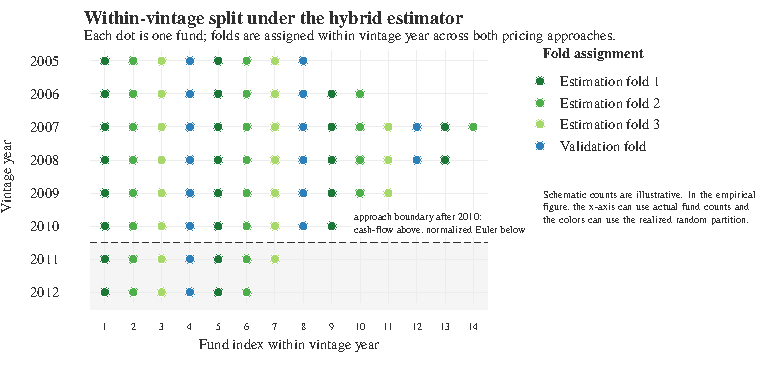
\includegraphics[width=\linewidth]{../figure/sampling_scheme_nav_pricing.pdf}
	\caption{Within-vintage fold assignment under the hybrid cash-flow / normalized-Euler estimator. Unseasoned vintages 2011--2012 (\(\mathcal V^U\), grey band) are included in estimation and validation like the seasoned vintages (\(\mathcal V^S\)), but contribute the normalized one-period Euler NAV error \(\epsilon^U\) in place of the cumulative cash-flow error \(\epsilon^S\).}
	\label{fig:nav-pricing-scheme}
\end{figure}

\subsection{Seasoned and unseasoned vintage sets}

Partition the active vintages into seasoned and unseasoned sets,
\[
\mathcal V = \mathcal V^S \cup \mathcal V^U.
\]
A vintage \(v\) is \emph{unseasoned} (\(v\in\mathcal V^U\)) if its aggregate residual NAV exceeds a fraction \(\delta\) of total committed capital; otherwise it is \emph{seasoned} (\(v\in\mathcal V^S\)). In practice, \(\delta\in[0.10,0.20]\) is a sensible range. For seasoned vintages, the pricing restriction is the standard cumulative cash-flow error as defined in Section~\ref{sec:pricing_moments}. For unseasoned vintages, we use the one-period Euler pricing error defined next and then normalize it into NPV-like per-committed-dollar units.

\subsection{One-period Euler pricing error}

For a fund \(i\) in an unseasoned vintage with quarterly NAV observations at dates \(t=0,1,\dots,T_i\), define the one-period pricing error for quarter \(t\):
\[
\eta_{t,i}(\theta)
=
\Psi_{t-1,t}(\theta)\cdot\bigl(CF_{t,i}+\mathrm{NAV}_{t,i}\bigr)
-\mathrm{NAV}_{t-1,i},
\]
where \(CF_{t,i}\) is the net cash flow during the quarter, \(\mathrm{NAV}_{t,i}\) is the reported net asset value at quarter-end, and \(\Psi_{t-1,t}(\theta)\) is the one-period stochastic discount factor.

The restriction \(E[\eta_{t,i}(\theta_0)]=0\) is an Euler equation: the beginning-of-period NAV equals the risk-adjusted present value of within-period distributions plus the end-of-period NAV. It is the same object that prices a one-period return on a traded asset, applied here to the NAV-implied gross return of the fund.

Any multiplicative factor known at date \(t-1\) preserves this moment restriction. This observation lets us turn \(\eta_{t,i}\) into a relative one-period pricing error without reintroducing cumulative discounting.

\subsection{Normalization and scale matching}

Define the lagged capital-at-risk scale
\[
s_{t-1,i}
=
\max\{\mathrm{NAV}_{t-1,i},\nu K_i\},
\qquad \nu\in[0.01,0.05],
\]
and the relative quarterly Euler error
\[
r_{t,i}(\theta)
=
\frac{\eta_{t,i}(\theta)}{s_{t-1,i}}.
\]
Because \(s_{t-1,i}\) is measurable at date \(t-1\), \(E[r_{t,i}(\theta_0)]=0\) whenever \(E[\eta_{t,i}(\theta_0)]=0\). The floor \(\nu K_i\) prevents the denominator from becoming arbitrarily small in the last few quarters of a nearly liquidated fund.

Next average within fund:
\[
\bar r_i(\theta)
=
\frac{1}{T_i}\sum_{t=1}^{T_i} r_{t,i}(\theta).
\]
This object is a mean quarterly pricing error per dollar at risk, but by itself it is too small in magnitude to be directly comparable to a seasoned NPV error accumulated over the life of the fund.

To map \(\bar r_i(\theta)\) into NPV-like units, let \(s(i)\) denote the strategy of fund \(i\), let \(\bar u_s(a)\) be a benchmark age-\(a\) profile of \(\mathrm{NAV}/K\) for strategy \(s\), and let \(q_{a-1}\) be a deterministic discount sequence (baseline \(q_{a-1}=1\), optional risk-free discounting as a robustness check). Define the duration-matching factor
\[
\Lambda_i
=
c_{s(i)}\sum_{a=1}^{T_i} q_{a-1}\,\bar u_{s(i)}(a),
\]
where \(c_{s(i)}\) is an optional strategy-specific calibration constant. In the simplest implementation \(c_{s(i)}=1\). If the raw duration scale still leaves systematic size gaps, \(c_{s(i)}\) can be chosen so that near-boundary seasoned and unseasoned funds have similar median absolute pricing moments within strategy.

The normalized unseasoned fund moment is
\[
g_i^U(\theta)
=
\Lambda_i\,\bar r_i(\theta),
\]
and for an unseasoned vintage \(v\in\mathcal V^U\) and fund cell \(C_{n,v,r}\), define the cell-level pricing error as
\[
\epsilon_{n,v,r}^{U}(\theta)
=
\frac{1}{|C_{n,v,r}|}
\sum_{i\in C_{n,v,r}} g_i^U(\theta).
\]

This normalization has a simple economic interpretation. The term \(\bar r_i(\theta)\) is the average quarterly pricing error per dollar at risk. The factor \(\Lambda_i\) is an externally chosen capital-at-risk duration: it measures how much \(\mathrm{NAV}/K\) exposure a typical fund of that age and strategy carries over its observed life. If the relative quarterly mispricing is roughly stable, \(r_{t,i}(\theta)\approx \rho_i(\theta)\), then
\[
g_i^U(\theta)\approx \rho_i(\theta)\,\Lambda_i,
\]
so the young-fund moment is of the same order as a life-of-fund NPV error per committed dollar. This is the sense in which the normalization is ``smart'': it matches scales without using the candidate cumulative SDF itself.

To diagnose whether the estimator disproportionately fits one group, the empirical implementation should report separate holdout losses for \(\mathcal V^S\) and \(\mathcal V^U\):
\[
S_n^S(M,\eta,\Pi)
=
L\!\left(\sum_{v\in\mathcal V^S\cap H_n}
\omega_{n,v,H_n}\,\epsilon^S_{n,v,H_n}(\hat\theta_n)\right),
\qquad
S_n^U(M,\eta,\Pi)
=
L\!\left(\sum_{v\in\mathcal V^U\cap H_n}
\omega_{n,v,H_n}\,\epsilon^U_{n,v,H_n}(\hat\theta_n)\right).
\]
If the average \(\bar S^U\) is systematically lower than \(\bar S^S\), the Euler restrictions are being trivially satisfied and contribute little to identification; if \(\bar S^U \gg \bar S^S\), the short NAV histories are dominating the holdout loss and the model selection may be driven by NAV fit rather than cash-flow fit.

\subsection{Why we do not discount to time zero}

Multiplying \(\eta_{t,i}(\theta)\) by \(\Psi_{0,t-1}(\theta)\) and summing would yield a valid moment, and for fully liquidated funds it would telescope. But for the young funds of actual interest it would recreate the long-horizon terminal-NAV term:
\[
\sum_{t=1}^{T_i}\Psi_{0,t-1}(\theta)\,\eta_{t,i}(\theta)
=
\sum_{t=1}^{T_i}\Psi_{0,t}(\theta)\,CF_{t,i}
\;+\;
\Psi_{0,T_i}(\theta)\,\mathrm{NAV}_{T_i,i}
\;-\;
\mathrm{NAV}_{0,i}.
\]
For an unseasoned fund, \(\mathrm{NAV}_{T_i,i}\neq 0\), so discounting the quarterly Euler errors back to time zero reconstructs exactly the large terminal-NAV present-value term that generates instability. The normalized construction above sacrifices path-by-path telescoping in order to preserve the short-horizon dependence of the young-fund block on the candidate SDF.

\subsection{Finite-sample role and asymptotic role}

The normalized Euler block has three useful consequences:
\begin{enumerate}
\item \textbf{Finite-sample stabilization.} Each quarterly Euler error depends on the one-period SDF only. The lagged scale \(s_{t-1,i}\) and duration factor \(\Lambda_i\) do not introduce additional candidate cumulative discounting. This keeps the sensitivity to \(\alpha\) proportional to quarter length rather than exponential in the fund horizon.
\item \textbf{Scale matching.} The factor \(\Lambda_i\) converts a mean quarterly relative Euler error into a cumulative NPV-like quantity per committed dollar. Young-vintage moments therefore have a magnitude comparable to seasoned NPV moments without appending a terminal NAV and discounting it over many years.
\item \textbf{Asymptotic irrelevance.} Only the most recent vintages within a bounded horizon \(D\) are classified as unseasoned. If \(\sup_i |\Lambda_i|<\infty\), then \(|\mathcal V^U|/V\to 0\) implies that the contribution of the normalized Euler block to the cross-vintage average vanishes. The estimator is therefore asymptotically cash-flow dominated, even though the young-vintage block is not algebraically identical to the seasoned NPV block.
\end{enumerate}

\paragraph{Remark: NAV quality and the Euler moment condition.}
The population Euler moment condition \(E[\eta_{t,i}(\theta_0)]=0\) makes a stronger claim: that the beginning-of-period NAV equals the risk-adjusted present value of within-period cash flows plus the end-of-period NAV. For traded assets, no-arbitrage forces this condition to hold. For private-equity funds, NAVs are appraisals whose co-movement with public factors may be smoothed or biased, so the Euler restriction holds only approximately.

The paper's design controls this concern in three ways. First, only unseasoned vintages rely on NAV-based moments; seasoned vintages are priced with realized cash flows alone. Second, even within \(\mathcal V^U\), the normalized Euler block uses one-quarter NAV changes and lagged scales rather than a single large terminal NAV discounted over many years. Third, the asymptotic irrelevance property ensures that the fraction of moment conditions relying on NAV quality vanishes as the panel grows.

\subsection{Why one-period restrictions stabilize alpha}

Under the standard cumulative approach, including an unseasoned fund with residual \(\mathrm{NAV}_T>0\) requires discounting by the cumulative SDF \(\Psi_{0,T}(\theta)\), which contains the factor \((1+\alpha)^{-T}\). For large \(T\) or large \(\mathrm{NAV}_T\), a small perturbation in \(\alpha\) produces a large swing in the pricing error. This mechanism could aggravate the exploding-alpha issue.

The quarterly Euler restriction replaces this single long-horizon discounting with \(T\) one-period discountings, each involving \((1+\alpha)^{-1}\). The sensitivity to \(\alpha\) is proportional to the quarter length \(\Delta t\), not exponential in the fund horizon \(T\). Moreover, the lagged scale \(s_{t-1,i}\) and duration factor \(\Lambda_i\) are fixed outside the candidate cumulative SDF, so the normalization does not reintroduce long-horizon alpha sensitivity. Each quarterly error \(\eta_{t,i}\) also subtracts \(\mathrm{NAV}_{t-1}\) from a discounted quantity of comparable magnitude, so the error is well-conditioned regardless of fund size.

\subsection{Integration into fold moments}

The fold moment retains its original form:
\[
m_{n,r}(\theta;M,\eta)
=
\sum_{v\in\mathcal V^S\cap A_{n,r}}
\omega_{n,v,r}\,\epsilon_{n,v,r}^{S}(\theta;M,\eta)
\;+\;
\sum_{v\in\mathcal V^U\cap A_{n,r}}
\omega_{n,v,r}\,\epsilon_{n,v,r}^{U}(\theta;M,\eta),
\]
where \(\epsilon^S\) is the standard cumulative cash-flow pricing error and \(\epsilon^U\) is the normalized Euler-based error defined above. Both terms are pricing errors that equal zero under correct pricing. The entire estimation and validation machinery from Sections~5 and~6 applies without modification---only the construction of vintage-level pricing errors differs between seasoned and unseasoned vintages.

\section{Relation to DLP12 and KN16}

The paper can be positioned in one paragraph:

\begin{itemize}
\item \textbf{From DLP12:} price private cash flows directly with an SDF.
\item \textbf{From KN16:} use aggregated pricing moments and an NPV-style abnormal-performance object.
\item \textbf{New here:} treat the construction of PE pricing moments as a resampling problem and rank SDF models by holdout pricing errors across many admissible fund assignments.
\item \textbf{Also new:} normalized Euler NAV restrictions for unseasoned vintages that retain short-horizon pricing information while matching the scale of seasoned cash-flow moments, avoiding both sample waste and exploding-alpha degeneracy (Section~\ref{sec:euler_nav}).
\end{itemize}

The paper is therefore not a repair of the existing SDF paper. It is a new empirical-design paper: how should we build, resample, and validate PE pricing moments when the sample is small and the moment construction is consequential?

\section{Empirical Algorithm}
\label{sec:algorithm}

For each candidate model \(M\), alpha design \(\eta\), and partition scheme \(\Pi\):

\begin{enumerate}
\item Partition vintages into seasoned (\(\mathcal V^S\)) and unseasoned (\(\mathcal V^U\)) sets (Section~\ref{sec:euler_nav}).
\item Choose \(P\) estimation folds and \(h\) holdout folds.
\item Draw a sampled assignment \(n\) from \(\Pi\).
\item Build fold cash-flow portfolios and fold pricing moments \(m_{n,r}(\theta;M,\eta)\).
\item Estimate \(\hat\theta_n(M,\eta,\Pi)\) on the \(P\) estimation folds.
\item Evaluate the fitted model on the holdout fold.
\item Repeat over many sampled assignments.
\item Rank model-design pairs by average holdout pricing loss.
\end{enumerate}

Alongside the mean holdout loss, report diagnostics that help interpret the ranking:

\begin{itemize}
\item median and dispersion of holdout losses,
\item dispersion of \(\hat\theta_n\) across assignments,
\item frequency of non-convergence,
\item frequency of boundary or exploding-alpha solutions,
\item sensitivity of results to within-vintage resampling versus shuffled vintage-year portfolios.
\end{itemize}

\bibliographystyle{plainnat}
\bibliography{resampling_refs}

\end{document}
